
%(BEGIN_QUESTION)
% Copyright 2010, Tony R. Kuphaldt, released under the Creative Commons Attribution License (v 1.0)
% This means you may do almost anything with this work of mine, so long as you give me proper credit

A safety device commonly installed on process vessels containing pressurized gases is a {\it Pressure Safety Valve}, or PSV.  In this example, a PSV protects a reactor vessel against rupture from excessive internal gas pressure, with the PSV set to open (``lift'') and vent the tank if the internal pressure exceeds 95 PSI:

$$\includegraphics[width=15.5cm]{i00765x01.eps}$$

Calculate the total force exerted on a 16 inch blind flange located on the side of the reactor at the PSV lift pressure, as well as the stress imposed by this force among the 20 bolts holding the flange in place, both answers expressed in the unit of {\it pounds}.  Use 15$1 \over 4$ inches as the effective diameter of the blind flange.

\vskip 10pt

$F_{total}$ = \underbar{\hskip 50pt} lb

\vskip 10pt

$F_{bolt}$ = \underbar{\hskip 50pt} lb


\vfil

\underbar{file i00765}
\eject
%(END_QUESTION)





%(BEGIN_ANSWER)

This is a graded question -- no answers or hints given!

%(END_ANSWER)





%(BEGIN_NOTES)

The pressure inside this vessel acts against the {\it effective} area of the flange.  Given an effective diameter of 15.25 inches, the effective area of this flange will be 182.65 square inches.  As a pressure of 95 PSI acts on this surface area, it generates a force on the flange equal to {\bf 17,352 pounds}.

\vskip 10pt

Assuming all 20 bolts holding this flange onto the vessel bear this force equally, each bolt will experience $1 \over 20$ of the force on the flange, or {\bf 867.6 pounds}.

%INDEX% Physics, fluids: pressure, force, and area
%INDEX% Physics, units and conversions: pressure
%INDEX% Safety, overpressure protection: safety valve

%(END_NOTES)


